% !TEX root = fig_architecture_standalone.tex
% =====================================================================
%  Standalone preview of fig_architecture.tex + fig_architecture_symbols.tex.
%
%  OVERLEAF: set this file as the Main document
%  (Menu -> Settings -> Main document, or right-click the file -> Set as
%  Main Document), then Recompile. Overleaf ALWAYS builds the main
%  document, never the tab you happen to have open. Set it back to your
%  thesis file afterwards.
%
%  For the thesis, put the \usepackage lines below into your own preamble
%  and use % =====================================================================
%  Figure: joint (chained) head architecture of MDNMixJoint.
%
%  Preamble requirements (both already present in model_lineage.tex;
%  methods.tex needs the two tikz lines adding):
%      \usepackage{amsmath}
%      \usepackage{graphicx}
%      \usepackage{tikz}
%      \usetikzlibrary{arrows.meta,positioning,fit,calc}
%
%  Use with:  % =====================================================================
%  Figure: joint (chained) head architecture of MDNMixJoint.
%
%  Preamble requirements (both already present in model_lineage.tex;
%  methods.tex needs the two tikz lines adding):
%      \usepackage{amsmath}
%      \usepackage{graphicx}
%      \usepackage{tikz}
%      \usetikzlibrary{arrows.meta,positioning,fit,calc}
%
%  Use with:  % =====================================================================
%  Figure: joint (chained) head architecture of MDNMixJoint.
%
%  Preamble requirements (both already present in model_lineage.tex;
%  methods.tex needs the two tikz lines adding):
%      \usepackage{amsmath}
%      \usepackage{graphicx}
%      \usepackage{tikz}
%      \usetikzlibrary{arrows.meta,positioning,fit,calc}
%
%  Use with:  \input{fig_architecture}
% =====================================================================
\begin{figure}[p]
\centering
\resizebox{\textwidth}{!}{%
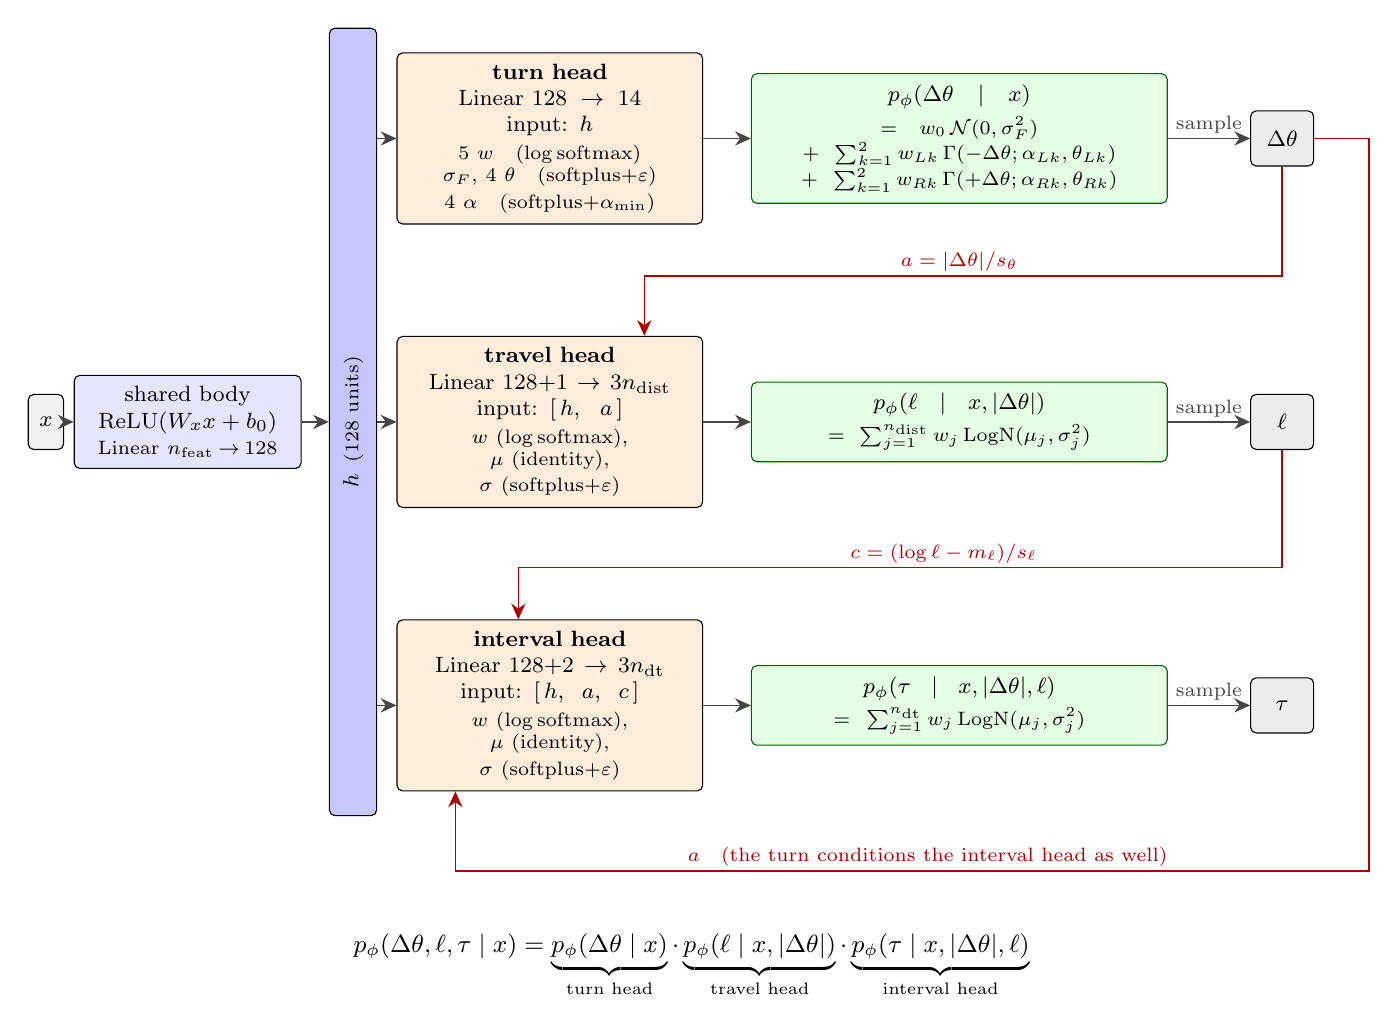
\begin{tikzpicture}[
  font=\footnotesize,
  >={Stealth[length=2mm,width=1.8mm]},
  bx/.style    = {draw, rounded corners=2pt, align=center, inner sep=4pt},
  inp/.style   = {bx, fill=gray!12, minimum height=7mm},
  bodyb/.style = {bx, fill=blue!10, text width=26mm},
  bar/.style   = {bx, fill=blue!22, minimum width=6mm, minimum height=100mm, inner sep=1pt},
  hd/.style    = {bx, fill=orange!14, text width=36mm},
  dn/.style    = {bx, fill=green!10, draw=green!40!black, text width=50mm},
  vl/.style    = {bx, fill=gray!15, minimum width=8mm, minimum height=7mm},
  fl/.style    = {->, semithick, gray!55!black},
  cd/.style    = {->, semithick, red!70!black},
  lb/.style    = {font=\scriptsize, inner sep=1.5pt},
]

% ---------------- shared trunk ----------------
\node[inp]   (x)  at (-6.2, 0) {$x$};
\node[bodyb] (bd) at (-4.4, 0) {shared body\\$\mathrm{ReLU}(W_x x + b_0)$\\
                                {\scriptsize Linear $n_{\mathrm{feat}}\!\to\!128$}};
\node[bar]   (b)  at (-2.3, 0) {\rotatebox{90}{$h$\, \scriptsize(128 units)}};

% ---------------- heads ----------------
\node[hd] (h1) at (0.2, 3.6) {\textbf{turn head}\\
  Linear $128 \to 14$\\
  input: $h$\\[2pt]
  {\scriptsize 5 $w$ \; ($\log\mathrm{softmax}$)\\
   $\sigma_F$, 4 $\theta$ \; ($\mathrm{softplus}{+}\varepsilon$)\\
   4 $\alpha$ \; ($\mathrm{softplus}{+}\alpha_{\min}$)}};
\node[hd] (h2) at (0.2, 0) {\textbf{travel head}\\
  Linear $128{+}1 \to 3n_{\mathrm{dist}}$\\
  input: $[\,h,\; a\,]$\\[2pt]
  {\scriptsize $w$ ($\log\mathrm{softmax}$), $\mu$ (identity),\\
   $\sigma$ ($\mathrm{softplus}{+}\varepsilon$)}};
\node[hd] (h3) at (0.2, -3.6) {\textbf{interval head}\\
  Linear $128{+}2 \to 3n_{\mathrm{dt}}$\\
  input: $[\,h,\; a,\; c\,]$\\[2pt]
  {\scriptsize $w$ ($\log\mathrm{softmax}$), $\mu$ (identity),\\
   $\sigma$ ($\mathrm{softplus}{+}\varepsilon$)}};

% ---------------- conditional densities ----------------
\node[dn] (d1) at (5.4, 3.6) {$p_\phi(\Delta\theta \mid x)$\\[2pt]
  {\scriptsize $= w_0\,\mathcal{N}(0,\sigma_F^2)$\\
   $+\;\sum_{k=1}^{2} w_{Lk}\,\Gamma(-\Delta\theta;\alpha_{Lk},\theta_{Lk})$\\
   $+\;\sum_{k=1}^{2} w_{Rk}\,\Gamma(+\Delta\theta;\alpha_{Rk},\theta_{Rk})$}};
\node[dn] (d2) at (5.4, 0) {$p_\phi(\ell \mid x, |\Delta\theta|)$\\[2pt]
  {\scriptsize $= \sum_{j=1}^{n_{\mathrm{dist}}} w_j\,\mathrm{LogN}(\mu_j,\sigma_j^2)$}};
\node[dn] (d3) at (5.4, -3.6) {$p_\phi(\tau \mid x, |\Delta\theta|, \ell)$\\[2pt]
  {\scriptsize $= \sum_{j=1}^{n_{\mathrm{dt}}} w_j\,\mathrm{LogN}(\mu_j,\sigma_j^2)$}};

% ---------------- emitted values ----------------
\node[vl] (v1) at (9.5, 3.6)  {$\Delta\theta$};
\node[vl] (v2) at (9.5, 0)    {$\ell$};
\node[vl] (v3) at (9.5, -3.6) {$\tau$};

% ---------------- trunk wiring ----------------
\draw[fl] (x) -- (bd);
\draw[fl] (bd) -- (b);
\draw[fl] (b.east |- h1) -- (h1.west);
\draw[fl] (b.east |- h2) -- (h2.west);
\draw[fl] (b.east |- h3) -- (h3.west);

\draw[fl] (h1.east) -- (d1.west);
\draw[fl] (h2.east) -- (d2.west);
\draw[fl] (h3.east) -- (d3.west);

\draw[fl] (d1.east) -- node[lb, above]{sample} (v1.west);
\draw[fl] (d2.east) -- node[lb, above]{sample} (v2.west);
\draw[fl] (d3.east) -- node[lb, above]{sample} (v3.west);

% ---------------- within-bout conditioners (the chain rule) ----------------
\draw[cd] (v1.south) -- (9.5,1.85) -- (1.4,1.85) -- (1.4,0 |- h2.north);
\node[lb, above, red!70!black] at (5.4,1.85) {$a = |\Delta\theta| / s_\theta$};

\draw[cd] (v2.south) -- (9.5,-1.85) -- (-0.2,-1.85) -- (-0.2,0 |- h3.north);
\node[lb, above, red!70!black] at (5.2,-1.85) {$c = (\log \ell - m_\ell)/s_\ell$};

\draw[cd] (v1.east) -- (10.6,3.6) -- (10.6,-5.7) -- (-1.0,-5.7) -- (-1.0,0 |- h3.south);
\node[lb, above, red!70!black] at (5.0,-5.7)
  {$a$ \; (the turn conditions the interval head as well)};

% ---------------- the factorisation ----------------
\node[align=center, font=\small] at (2.0,-6.9)
  {$p_\phi(\Delta\theta,\ell,\tau \mid x)
    = \underbrace{p_\phi(\Delta\theta \mid x)}_{\text{turn head}}
    \cdot \underbrace{p_\phi(\ell \mid x, |\Delta\theta|)}_{\text{travel head}}
    \cdot \underbrace{p_\phi(\tau \mid x, |\Delta\theta|, \ell)}_{\text{interval head}}$};

\end{tikzpicture}}
\caption{\textbf{Chained head architecture and the joint density it defines.}
One shared hidden layer maps the feature vector $x$ to the body representation $h$, which
every head reads. The heads do not emit probabilities: each emits the \emph{parameters} of
one conditional density (orange $\to$ green), and the joint is the chain-rule product of
the three. The red wires are the within-bout conditioners --- the travel head additionally
receives the absolute turn $a=|\Delta\theta|/s_\theta$, and the interval head receives that
and the centred log travel distance $c=(\log\ell-m_\ell)/s_\ell$, each rescaled exactly as
the corresponding history block is. During \emph{training} the red wires are teacher-forced
from the observed bout, so the three log-densities sum to the exact log joint and the loss
is $-\big[\log p_\phi(\Delta\theta\mid x)+\log p_\phi(\ell\mid x,|\Delta\theta|)
+\log p_\phi(\tau\mid x,|\Delta\theta|,\ell)\big]$ --- no bound and no approximation.
During \emph{sampling} the same wires carry the model's own draws, so a bout is generated
ancestrally, top to bottom. Only the sign-free $|\Delta\theta|$ is passed: left and right
must not change step size or timing, and feeding the sign would break the symmetry the
angle mixture enforces.}
\label{fig:architecture}
\end{figure}

% =====================================================================
\begin{figure}[p]
\centering
\resizebox{\textwidth}{!}{%
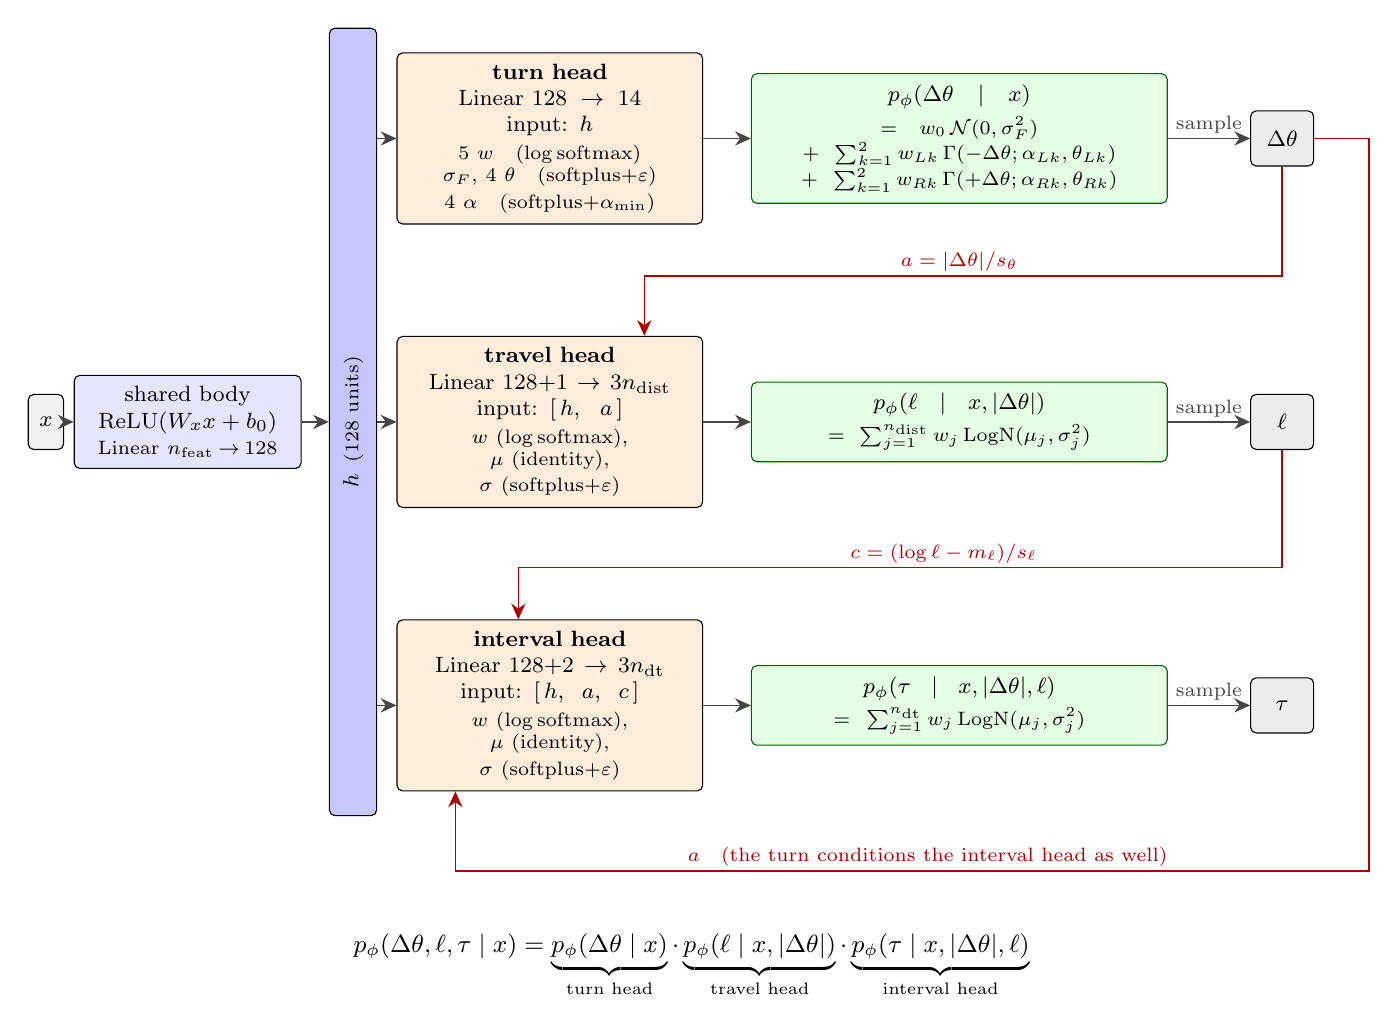
\begin{tikzpicture}[
  font=\footnotesize,
  >={Stealth[length=2mm,width=1.8mm]},
  bx/.style    = {draw, rounded corners=2pt, align=center, inner sep=4pt},
  inp/.style   = {bx, fill=gray!12, minimum height=7mm},
  bodyb/.style = {bx, fill=blue!10, text width=26mm},
  bar/.style   = {bx, fill=blue!22, minimum width=6mm, minimum height=100mm, inner sep=1pt},
  hd/.style    = {bx, fill=orange!14, text width=36mm},
  dn/.style    = {bx, fill=green!10, draw=green!40!black, text width=50mm},
  vl/.style    = {bx, fill=gray!15, minimum width=8mm, minimum height=7mm},
  fl/.style    = {->, semithick, gray!55!black},
  cd/.style    = {->, semithick, red!70!black},
  lb/.style    = {font=\scriptsize, inner sep=1.5pt},
]

% ---------------- shared trunk ----------------
\node[inp]   (x)  at (-6.2, 0) {$x$};
\node[bodyb] (bd) at (-4.4, 0) {shared body\\$\mathrm{ReLU}(W_x x + b_0)$\\
                                {\scriptsize Linear $n_{\mathrm{feat}}\!\to\!128$}};
\node[bar]   (b)  at (-2.3, 0) {\rotatebox{90}{$h$\, \scriptsize(128 units)}};

% ---------------- heads ----------------
\node[hd] (h1) at (0.2, 3.6) {\textbf{turn head}\\
  Linear $128 \to 14$\\
  input: $h$\\[2pt]
  {\scriptsize 5 $w$ \; ($\log\mathrm{softmax}$)\\
   $\sigma_F$, 4 $\theta$ \; ($\mathrm{softplus}{+}\varepsilon$)\\
   4 $\alpha$ \; ($\mathrm{softplus}{+}\alpha_{\min}$)}};
\node[hd] (h2) at (0.2, 0) {\textbf{travel head}\\
  Linear $128{+}1 \to 3n_{\mathrm{dist}}$\\
  input: $[\,h,\; a\,]$\\[2pt]
  {\scriptsize $w$ ($\log\mathrm{softmax}$), $\mu$ (identity),\\
   $\sigma$ ($\mathrm{softplus}{+}\varepsilon$)}};
\node[hd] (h3) at (0.2, -3.6) {\textbf{interval head}\\
  Linear $128{+}2 \to 3n_{\mathrm{dt}}$\\
  input: $[\,h,\; a,\; c\,]$\\[2pt]
  {\scriptsize $w$ ($\log\mathrm{softmax}$), $\mu$ (identity),\\
   $\sigma$ ($\mathrm{softplus}{+}\varepsilon$)}};

% ---------------- conditional densities ----------------
\node[dn] (d1) at (5.4, 3.6) {$p_\phi(\Delta\theta \mid x)$\\[2pt]
  {\scriptsize $= w_0\,\mathcal{N}(0,\sigma_F^2)$\\
   $+\;\sum_{k=1}^{2} w_{Lk}\,\Gamma(-\Delta\theta;\alpha_{Lk},\theta_{Lk})$\\
   $+\;\sum_{k=1}^{2} w_{Rk}\,\Gamma(+\Delta\theta;\alpha_{Rk},\theta_{Rk})$}};
\node[dn] (d2) at (5.4, 0) {$p_\phi(\ell \mid x, |\Delta\theta|)$\\[2pt]
  {\scriptsize $= \sum_{j=1}^{n_{\mathrm{dist}}} w_j\,\mathrm{LogN}(\mu_j,\sigma_j^2)$}};
\node[dn] (d3) at (5.4, -3.6) {$p_\phi(\tau \mid x, |\Delta\theta|, \ell)$\\[2pt]
  {\scriptsize $= \sum_{j=1}^{n_{\mathrm{dt}}} w_j\,\mathrm{LogN}(\mu_j,\sigma_j^2)$}};

% ---------------- emitted values ----------------
\node[vl] (v1) at (9.5, 3.6)  {$\Delta\theta$};
\node[vl] (v2) at (9.5, 0)    {$\ell$};
\node[vl] (v3) at (9.5, -3.6) {$\tau$};

% ---------------- trunk wiring ----------------
\draw[fl] (x) -- (bd);
\draw[fl] (bd) -- (b);
\draw[fl] (b.east |- h1) -- (h1.west);
\draw[fl] (b.east |- h2) -- (h2.west);
\draw[fl] (b.east |- h3) -- (h3.west);

\draw[fl] (h1.east) -- (d1.west);
\draw[fl] (h2.east) -- (d2.west);
\draw[fl] (h3.east) -- (d3.west);

\draw[fl] (d1.east) -- node[lb, above]{sample} (v1.west);
\draw[fl] (d2.east) -- node[lb, above]{sample} (v2.west);
\draw[fl] (d3.east) -- node[lb, above]{sample} (v3.west);

% ---------------- within-bout conditioners (the chain rule) ----------------
\draw[cd] (v1.south) -- (9.5,1.85) -- (1.4,1.85) -- (1.4,0 |- h2.north);
\node[lb, above, red!70!black] at (5.4,1.85) {$a = |\Delta\theta| / s_\theta$};

\draw[cd] (v2.south) -- (9.5,-1.85) -- (-0.2,-1.85) -- (-0.2,0 |- h3.north);
\node[lb, above, red!70!black] at (5.2,-1.85) {$c = (\log \ell - m_\ell)/s_\ell$};

\draw[cd] (v1.east) -- (10.6,3.6) -- (10.6,-5.7) -- (-1.0,-5.7) -- (-1.0,0 |- h3.south);
\node[lb, above, red!70!black] at (5.0,-5.7)
  {$a$ \; (the turn conditions the interval head as well)};

% ---------------- the factorisation ----------------
\node[align=center, font=\small] at (2.0,-6.9)
  {$p_\phi(\Delta\theta,\ell,\tau \mid x)
    = \underbrace{p_\phi(\Delta\theta \mid x)}_{\text{turn head}}
    \cdot \underbrace{p_\phi(\ell \mid x, |\Delta\theta|)}_{\text{travel head}}
    \cdot \underbrace{p_\phi(\tau \mid x, |\Delta\theta|, \ell)}_{\text{interval head}}$};

\end{tikzpicture}}
\caption{\textbf{Chained head architecture and the joint density it defines.}
One shared hidden layer maps the feature vector $x$ to the body representation $h$, which
every head reads. The heads do not emit probabilities: each emits the \emph{parameters} of
one conditional density (orange $\to$ green), and the joint is the chain-rule product of
the three. The red wires are the within-bout conditioners --- the travel head additionally
receives the absolute turn $a=|\Delta\theta|/s_\theta$, and the interval head receives that
and the centred log travel distance $c=(\log\ell-m_\ell)/s_\ell$, each rescaled exactly as
the corresponding history block is. During \emph{training} the red wires are teacher-forced
from the observed bout, so the three log-densities sum to the exact log joint and the loss
is $-\big[\log p_\phi(\Delta\theta\mid x)+\log p_\phi(\ell\mid x,|\Delta\theta|)
+\log p_\phi(\tau\mid x,|\Delta\theta|,\ell)\big]$ --- no bound and no approximation.
During \emph{sampling} the same wires carry the model's own draws, so a bout is generated
ancestrally, top to bottom. Only the sign-free $|\Delta\theta|$ is passed: left and right
must not change step size or timing, and feeding the sign would break the symmetry the
angle mixture enforces.}
\label{fig:architecture}
\end{figure}

% =====================================================================
\begin{figure}[p]
\centering
\resizebox{\textwidth}{!}{%
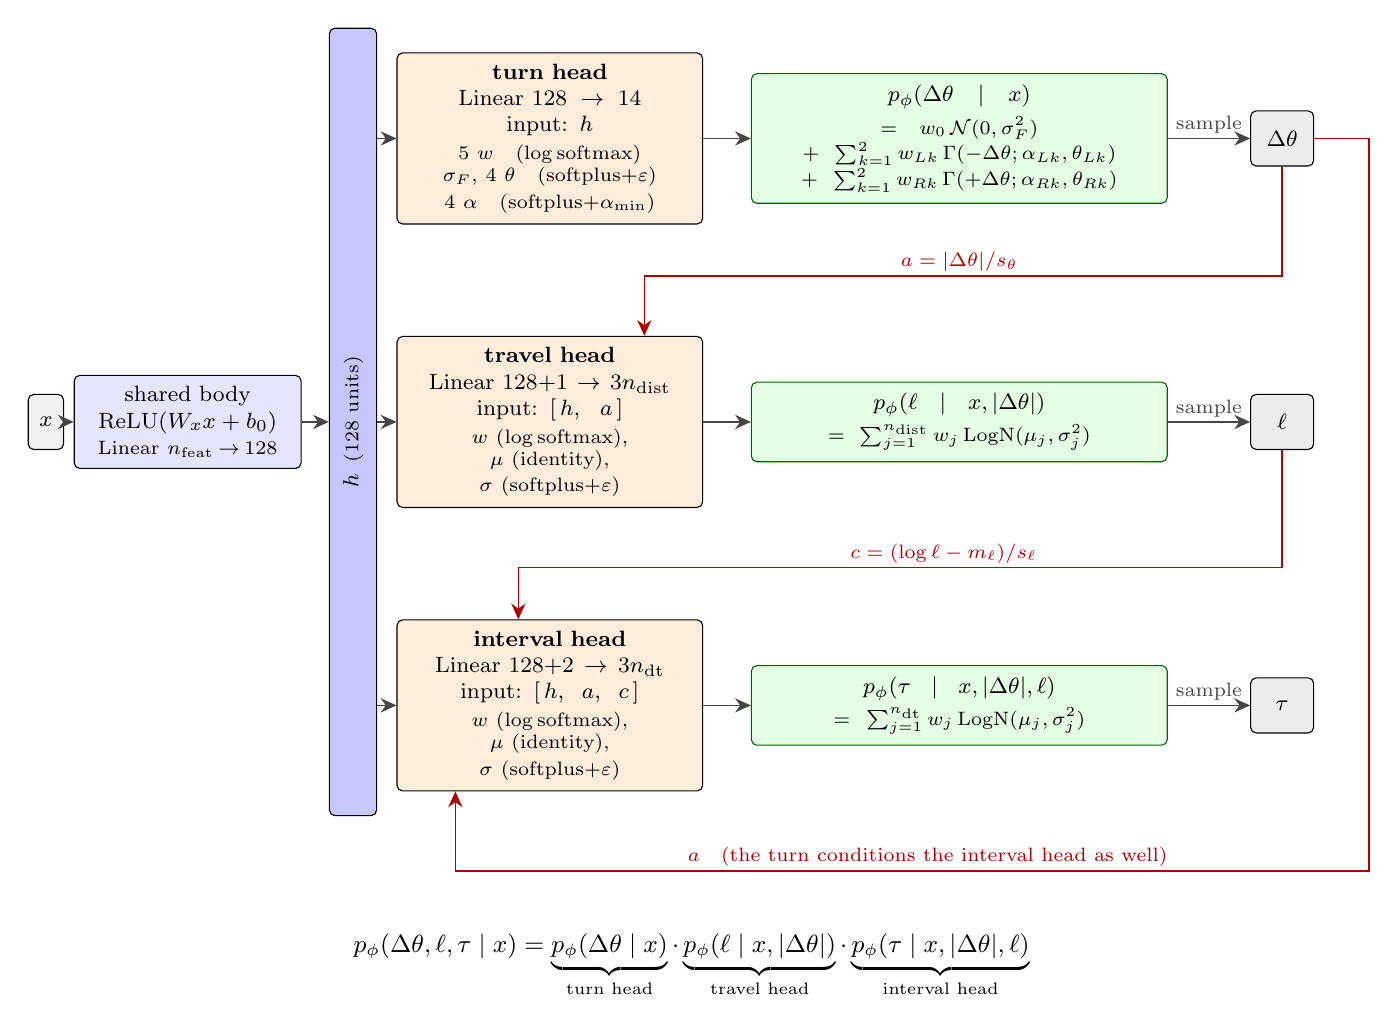
\begin{tikzpicture}[
  font=\footnotesize,
  >={Stealth[length=2mm,width=1.8mm]},
  bx/.style    = {draw, rounded corners=2pt, align=center, inner sep=4pt},
  inp/.style   = {bx, fill=gray!12, minimum height=7mm},
  bodyb/.style = {bx, fill=blue!10, text width=26mm},
  bar/.style   = {bx, fill=blue!22, minimum width=6mm, minimum height=100mm, inner sep=1pt},
  hd/.style    = {bx, fill=orange!14, text width=36mm},
  dn/.style    = {bx, fill=green!10, draw=green!40!black, text width=50mm},
  vl/.style    = {bx, fill=gray!15, minimum width=8mm, minimum height=7mm},
  fl/.style    = {->, semithick, gray!55!black},
  cd/.style    = {->, semithick, red!70!black},
  lb/.style    = {font=\scriptsize, inner sep=1.5pt},
]

% ---------------- shared trunk ----------------
\node[inp]   (x)  at (-6.2, 0) {$x$};
\node[bodyb] (bd) at (-4.4, 0) {shared body\\$\mathrm{ReLU}(W_x x + b_0)$\\
                                {\scriptsize Linear $n_{\mathrm{feat}}\!\to\!128$}};
\node[bar]   (b)  at (-2.3, 0) {\rotatebox{90}{$h$\, \scriptsize(128 units)}};

% ---------------- heads ----------------
\node[hd] (h1) at (0.2, 3.6) {\textbf{turn head}\\
  Linear $128 \to 14$\\
  input: $h$\\[2pt]
  {\scriptsize 5 $w$ \; ($\log\mathrm{softmax}$)\\
   $\sigma_F$, 4 $\theta$ \; ($\mathrm{softplus}{+}\varepsilon$)\\
   4 $\alpha$ \; ($\mathrm{softplus}{+}\alpha_{\min}$)}};
\node[hd] (h2) at (0.2, 0) {\textbf{travel head}\\
  Linear $128{+}1 \to 3n_{\mathrm{dist}}$\\
  input: $[\,h,\; a\,]$\\[2pt]
  {\scriptsize $w$ ($\log\mathrm{softmax}$), $\mu$ (identity),\\
   $\sigma$ ($\mathrm{softplus}{+}\varepsilon$)}};
\node[hd] (h3) at (0.2, -3.6) {\textbf{interval head}\\
  Linear $128{+}2 \to 3n_{\mathrm{dt}}$\\
  input: $[\,h,\; a,\; c\,]$\\[2pt]
  {\scriptsize $w$ ($\log\mathrm{softmax}$), $\mu$ (identity),\\
   $\sigma$ ($\mathrm{softplus}{+}\varepsilon$)}};

% ---------------- conditional densities ----------------
\node[dn] (d1) at (5.4, 3.6) {$p_\phi(\Delta\theta \mid x)$\\[2pt]
  {\scriptsize $= w_0\,\mathcal{N}(0,\sigma_F^2)$\\
   $+\;\sum_{k=1}^{2} w_{Lk}\,\Gamma(-\Delta\theta;\alpha_{Lk},\theta_{Lk})$\\
   $+\;\sum_{k=1}^{2} w_{Rk}\,\Gamma(+\Delta\theta;\alpha_{Rk},\theta_{Rk})$}};
\node[dn] (d2) at (5.4, 0) {$p_\phi(\ell \mid x, |\Delta\theta|)$\\[2pt]
  {\scriptsize $= \sum_{j=1}^{n_{\mathrm{dist}}} w_j\,\mathrm{LogN}(\mu_j,\sigma_j^2)$}};
\node[dn] (d3) at (5.4, -3.6) {$p_\phi(\tau \mid x, |\Delta\theta|, \ell)$\\[2pt]
  {\scriptsize $= \sum_{j=1}^{n_{\mathrm{dt}}} w_j\,\mathrm{LogN}(\mu_j,\sigma_j^2)$}};

% ---------------- emitted values ----------------
\node[vl] (v1) at (9.5, 3.6)  {$\Delta\theta$};
\node[vl] (v2) at (9.5, 0)    {$\ell$};
\node[vl] (v3) at (9.5, -3.6) {$\tau$};

% ---------------- trunk wiring ----------------
\draw[fl] (x) -- (bd);
\draw[fl] (bd) -- (b);
\draw[fl] (b.east |- h1) -- (h1.west);
\draw[fl] (b.east |- h2) -- (h2.west);
\draw[fl] (b.east |- h3) -- (h3.west);

\draw[fl] (h1.east) -- (d1.west);
\draw[fl] (h2.east) -- (d2.west);
\draw[fl] (h3.east) -- (d3.west);

\draw[fl] (d1.east) -- node[lb, above]{sample} (v1.west);
\draw[fl] (d2.east) -- node[lb, above]{sample} (v2.west);
\draw[fl] (d3.east) -- node[lb, above]{sample} (v3.west);

% ---------------- within-bout conditioners (the chain rule) ----------------
\draw[cd] (v1.south) -- (9.5,1.85) -- (1.4,1.85) -- (1.4,0 |- h2.north);
\node[lb, above, red!70!black] at (5.4,1.85) {$a = |\Delta\theta| / s_\theta$};

\draw[cd] (v2.south) -- (9.5,-1.85) -- (-0.2,-1.85) -- (-0.2,0 |- h3.north);
\node[lb, above, red!70!black] at (5.2,-1.85) {$c = (\log \ell - m_\ell)/s_\ell$};

\draw[cd] (v1.east) -- (10.6,3.6) -- (10.6,-5.7) -- (-1.0,-5.7) -- (-1.0,0 |- h3.south);
\node[lb, above, red!70!black] at (5.0,-5.7)
  {$a$ \; (the turn conditions the interval head as well)};

% ---------------- the factorisation ----------------
\node[align=center, font=\small] at (2.0,-6.9)
  {$p_\phi(\Delta\theta,\ell,\tau \mid x)
    = \underbrace{p_\phi(\Delta\theta \mid x)}_{\text{turn head}}
    \cdot \underbrace{p_\phi(\ell \mid x, |\Delta\theta|)}_{\text{travel head}}
    \cdot \underbrace{p_\phi(\tau \mid x, |\Delta\theta|, \ell)}_{\text{interval head}}$};

\end{tikzpicture}}
\caption{\textbf{Chained head architecture and the joint density it defines.}
One shared hidden layer maps the feature vector $x$ to the body representation $h$, which
every head reads. The heads do not emit probabilities: each emits the \emph{parameters} of
one conditional density (orange $\to$ green), and the joint is the chain-rule product of
the three. The red wires are the within-bout conditioners --- the travel head additionally
receives the absolute turn $a=|\Delta\theta|/s_\theta$, and the interval head receives that
and the centred log travel distance $c=(\log\ell-m_\ell)/s_\ell$, each rescaled exactly as
the corresponding history block is. During \emph{training} the red wires are teacher-forced
from the observed bout, so the three log-densities sum to the exact log joint and the loss
is $-\big[\log p_\phi(\Delta\theta\mid x)+\log p_\phi(\ell\mid x,|\Delta\theta|)
+\log p_\phi(\tau\mid x,|\Delta\theta|,\ell)\big]$ --- no bound and no approximation.
During \emph{sampling} the same wires carry the model's own draws, so a bout is generated
ancestrally, top to bottom. Only the sign-free $|\Delta\theta|$ is passed: left and right
must not change step size or timing, and feeding the sign would break the symmetry the
angle mixture enforces.}
\label{fig:architecture}
\end{figure}
 / % =====================================================================
%  Nomenclature for fig_architecture.tex.
%  Requires: \usepackage{booktabs}  \usepackage{array}  \usepackage{amsmath}
%  Use with: % =====================================================================
%  Nomenclature for fig_architecture.tex.
%  Requires: \usepackage{booktabs}  \usepackage{array}  \usepackage{amsmath}
%  Use with: % =====================================================================
%  Nomenclature for fig_architecture.tex.
%  Requires: \usepackage{booktabs}  \usepackage{array}  \usepackage{amsmath}
%  Use with: \input{fig_architecture_symbols}
% =====================================================================
\begin{table}[t]
\centering\small
\renewcommand{\arraystretch}{1.18}
\begin{tabular}{@{}l l p{0.56\linewidth}@{}}
\toprule
\textbf{symbol} & \textbf{space} & \textbf{meaning}\\
\midrule
\multicolumn{3}{@{}l}{\emph{Shared trunk}}\\
$x$        & $\mathbb{R}^{n_{\mathrm{feat}}}$ & input feature vector for one bout: the
             concatenated turn-history, symbol, stimulus, border, adaptation and
             kinematic-history blocks; $n_{\mathrm{feat}}$ is their total width\\
$W_x$      & $\mathbb{R}^{128\times n_{\mathrm{feat}}}$ & weight matrix of the single hidden layer\\
$b_0$      & $\mathbb{R}^{128}$ & bias vector of that layer\\
$h$        & $\mathbb{R}^{128}$ & hidden (body) representation $h=\mathrm{ReLU}(W_x x + b_0)$,
             read by all three heads; $128$ is the layer width\\
$\phi$     & --- & all trainable parameters ($W_x$, $b_0$ and the three head weight matrices
             and biases); the subscript in $p_\phi$\\
\addlinespace
\multicolumn{3}{@{}l}{\emph{The three emitted channels of a bout}}\\
$\Delta\theta$ & $(-180,180]$ deg & signed reorientation angle (the turn)\\
$\ell$     & $(0,\infty)$ px & travel distance of the bout, onset to onset\\
$\tau$     & $(0,\infty)$ s  & inter-bout interval\\
\addlinespace
\multicolumn{3}{@{}l}{\emph{Within-bout conditioners (the chain-rule wires)}}\\
$a$        & $\mathbb{R}_{\ge 0}$ & rescaled absolute turn, $a=|\Delta\theta|/s_\theta$\\
$c$        & $\mathbb{R}$ & centred log travel distance, $c=(\log\ell-m_\ell)/s_\ell$\\
$s_\theta$ & $>0$ & turn scale, $\max(\mathrm{sd}(\Delta\theta),1)$ on the training fold\\
$m_\ell,\,s_\ell$ & $\mathbb{R},>0$ & mean and sd of $\log\ell$ on the training fold\\
\addlinespace
\multicolumn{3}{@{}l}{\emph{Turn-head parameters (14 raw outputs)}}\\
$w_0,w_{L1},w_{L2},w_{R1},w_{R2}$ & simplex & the five mixture weights ($\log\mathrm{softmax}$)\\
$\sigma_F$ & $>0$ & standard deviation of the forward Normal, centred at $0$\\
$\alpha_{Lk},\theta_{Lk}$ & $\ge\alpha_{\min},>0$ & shape and scale of left Gamma $k$, on $-\Delta\theta$\\
$\alpha_{Rk},\theta_{Rk}$ & $\ge\alpha_{\min},>0$ & shape and scale of right Gamma $k$, on $+\Delta\theta$\\
\addlinespace
\multicolumn{3}{@{}l}{\emph{Travel- and interval-head parameters}}\\
$n_{\mathrm{dist}},\,n_{\mathrm{dt}}$ & $\mathbb{N}$ & number of log-normal components (2 and 3)\\
$w_j,\mu_j,\sigma_j$ & simplex, $\mathbb{R}$, $>0$ & weight, log-scale location and log-scale
             spread of component $j$; $3n$ raw outputs per head\\
\addlinespace
\multicolumn{3}{@{}l}{\emph{Constants and distributions}}\\
$\varepsilon$ & $10^{-12}$ & softplus floor keeping every scale strictly positive\\
$\alpha_{\min}$ & $1$ & floor on the Gamma shape, so no component diverges at $\Delta\theta\!\to\!0$\\
$\mathcal{N}(0,\sigma^2)$ & --- & Normal density\\
$\Gamma(u;\alpha,\theta)$ & --- & Gamma density on $u>0$, shape $\alpha$, scale $\theta$\\
$\mathrm{LogN}(\mu,\sigma^2)$ & --- & log-normal: $\log X\sim\mathcal{N}(\mu,\sigma^2)$\\
\bottomrule
\end{tabular}
\caption{Symbols used in Fig.~\ref{fig:architecture}.}
\label{tab:architecture-symbols}
\end{table}

% =====================================================================
\begin{table}[t]
\centering\small
\renewcommand{\arraystretch}{1.18}
\begin{tabular}{@{}l l p{0.56\linewidth}@{}}
\toprule
\textbf{symbol} & \textbf{space} & \textbf{meaning}\\
\midrule
\multicolumn{3}{@{}l}{\emph{Shared trunk}}\\
$x$        & $\mathbb{R}^{n_{\mathrm{feat}}}$ & input feature vector for one bout: the
             concatenated turn-history, symbol, stimulus, border, adaptation and
             kinematic-history blocks; $n_{\mathrm{feat}}$ is their total width\\
$W_x$      & $\mathbb{R}^{128\times n_{\mathrm{feat}}}$ & weight matrix of the single hidden layer\\
$b_0$      & $\mathbb{R}^{128}$ & bias vector of that layer\\
$h$        & $\mathbb{R}^{128}$ & hidden (body) representation $h=\mathrm{ReLU}(W_x x + b_0)$,
             read by all three heads; $128$ is the layer width\\
$\phi$     & --- & all trainable parameters ($W_x$, $b_0$ and the three head weight matrices
             and biases); the subscript in $p_\phi$\\
\addlinespace
\multicolumn{3}{@{}l}{\emph{The three emitted channels of a bout}}\\
$\Delta\theta$ & $(-180,180]$ deg & signed reorientation angle (the turn)\\
$\ell$     & $(0,\infty)$ px & travel distance of the bout, onset to onset\\
$\tau$     & $(0,\infty)$ s  & inter-bout interval\\
\addlinespace
\multicolumn{3}{@{}l}{\emph{Within-bout conditioners (the chain-rule wires)}}\\
$a$        & $\mathbb{R}_{\ge 0}$ & rescaled absolute turn, $a=|\Delta\theta|/s_\theta$\\
$c$        & $\mathbb{R}$ & centred log travel distance, $c=(\log\ell-m_\ell)/s_\ell$\\
$s_\theta$ & $>0$ & turn scale, $\max(\mathrm{sd}(\Delta\theta),1)$ on the training fold\\
$m_\ell,\,s_\ell$ & $\mathbb{R},>0$ & mean and sd of $\log\ell$ on the training fold\\
\addlinespace
\multicolumn{3}{@{}l}{\emph{Turn-head parameters (14 raw outputs)}}\\
$w_0,w_{L1},w_{L2},w_{R1},w_{R2}$ & simplex & the five mixture weights ($\log\mathrm{softmax}$)\\
$\sigma_F$ & $>0$ & standard deviation of the forward Normal, centred at $0$\\
$\alpha_{Lk},\theta_{Lk}$ & $\ge\alpha_{\min},>0$ & shape and scale of left Gamma $k$, on $-\Delta\theta$\\
$\alpha_{Rk},\theta_{Rk}$ & $\ge\alpha_{\min},>0$ & shape and scale of right Gamma $k$, on $+\Delta\theta$\\
\addlinespace
\multicolumn{3}{@{}l}{\emph{Travel- and interval-head parameters}}\\
$n_{\mathrm{dist}},\,n_{\mathrm{dt}}$ & $\mathbb{N}$ & number of log-normal components (2 and 3)\\
$w_j,\mu_j,\sigma_j$ & simplex, $\mathbb{R}$, $>0$ & weight, log-scale location and log-scale
             spread of component $j$; $3n$ raw outputs per head\\
\addlinespace
\multicolumn{3}{@{}l}{\emph{Constants and distributions}}\\
$\varepsilon$ & $10^{-12}$ & softplus floor keeping every scale strictly positive\\
$\alpha_{\min}$ & $1$ & floor on the Gamma shape, so no component diverges at $\Delta\theta\!\to\!0$\\
$\mathcal{N}(0,\sigma^2)$ & --- & Normal density\\
$\Gamma(u;\alpha,\theta)$ & --- & Gamma density on $u>0$, shape $\alpha$, scale $\theta$\\
$\mathrm{LogN}(\mu,\sigma^2)$ & --- & log-normal: $\log X\sim\mathcal{N}(\mu,\sigma^2)$\\
\bottomrule
\end{tabular}
\caption{Symbols used in Fig.~\ref{fig:architecture}.}
\label{tab:architecture-symbols}
\end{table}

% =====================================================================
\begin{table}[t]
\centering\small
\renewcommand{\arraystretch}{1.18}
\begin{tabular}{@{}l l p{0.56\linewidth}@{}}
\toprule
\textbf{symbol} & \textbf{space} & \textbf{meaning}\\
\midrule
\multicolumn{3}{@{}l}{\emph{Shared trunk}}\\
$x$        & $\mathbb{R}^{n_{\mathrm{feat}}}$ & input feature vector for one bout: the
             concatenated turn-history, symbol, stimulus, border, adaptation and
             kinematic-history blocks; $n_{\mathrm{feat}}$ is their total width\\
$W_x$      & $\mathbb{R}^{128\times n_{\mathrm{feat}}}$ & weight matrix of the single hidden layer\\
$b_0$      & $\mathbb{R}^{128}$ & bias vector of that layer\\
$h$        & $\mathbb{R}^{128}$ & hidden (body) representation $h=\mathrm{ReLU}(W_x x + b_0)$,
             read by all three heads; $128$ is the layer width\\
$\phi$     & --- & all trainable parameters ($W_x$, $b_0$ and the three head weight matrices
             and biases); the subscript in $p_\phi$\\
\addlinespace
\multicolumn{3}{@{}l}{\emph{The three emitted channels of a bout}}\\
$\Delta\theta$ & $(-180,180]$ deg & signed reorientation angle (the turn)\\
$\ell$     & $(0,\infty)$ px & travel distance of the bout, onset to onset\\
$\tau$     & $(0,\infty)$ s  & inter-bout interval\\
\addlinespace
\multicolumn{3}{@{}l}{\emph{Within-bout conditioners (the chain-rule wires)}}\\
$a$        & $\mathbb{R}_{\ge 0}$ & rescaled absolute turn, $a=|\Delta\theta|/s_\theta$\\
$c$        & $\mathbb{R}$ & centred log travel distance, $c=(\log\ell-m_\ell)/s_\ell$\\
$s_\theta$ & $>0$ & turn scale, $\max(\mathrm{sd}(\Delta\theta),1)$ on the training fold\\
$m_\ell,\,s_\ell$ & $\mathbb{R},>0$ & mean and sd of $\log\ell$ on the training fold\\
\addlinespace
\multicolumn{3}{@{}l}{\emph{Turn-head parameters (14 raw outputs)}}\\
$w_0,w_{L1},w_{L2},w_{R1},w_{R2}$ & simplex & the five mixture weights ($\log\mathrm{softmax}$)\\
$\sigma_F$ & $>0$ & standard deviation of the forward Normal, centred at $0$\\
$\alpha_{Lk},\theta_{Lk}$ & $\ge\alpha_{\min},>0$ & shape and scale of left Gamma $k$, on $-\Delta\theta$\\
$\alpha_{Rk},\theta_{Rk}$ & $\ge\alpha_{\min},>0$ & shape and scale of right Gamma $k$, on $+\Delta\theta$\\
\addlinespace
\multicolumn{3}{@{}l}{\emph{Travel- and interval-head parameters}}\\
$n_{\mathrm{dist}},\,n_{\mathrm{dt}}$ & $\mathbb{N}$ & number of log-normal components (2 and 3)\\
$w_j,\mu_j,\sigma_j$ & simplex, $\mathbb{R}$, $>0$ & weight, log-scale location and log-scale
             spread of component $j$; $3n$ raw outputs per head\\
\addlinespace
\multicolumn{3}{@{}l}{\emph{Constants and distributions}}\\
$\varepsilon$ & $10^{-12}$ & softplus floor keeping every scale strictly positive\\
$\alpha_{\min}$ & $1$ & floor on the Gamma shape, so no component diverges at $\Delta\theta\!\to\!0$\\
$\mathcal{N}(0,\sigma^2)$ & --- & Normal density\\
$\Gamma(u;\alpha,\theta)$ & --- & Gamma density on $u>0$, shape $\alpha$, scale $\theta$\\
$\mathrm{LogN}(\mu,\sigma^2)$ & --- & log-normal: $\log X\sim\mathcal{N}(\mu,\sigma^2)$\\
\bottomrule
\end{tabular}
\caption{Symbols used in Fig.~\ref{fig:architecture}.}
\label{tab:architecture-symbols}
\end{table}

%  where the figure and table belong.
% =====================================================================
\documentclass[11pt,a4paper]{article}
\usepackage[T1]{fontenc}
\usepackage[utf8]{inputenc}
\usepackage[margin=2.4cm]{geometry}
\usepackage{amsmath,amssymb}
\usepackage{booktabs}
\usepackage{array}
\usepackage{xcolor}
\usepackage{graphicx}
\usepackage{tikz}
\usetikzlibrary{arrows.meta,positioning,fit,calc}

\pagestyle{empty}

\begin{document}

% =====================================================================
%  Figure: joint (chained) head architecture of MDNMixJoint.
%
%  Preamble requirements (both already present in model_lineage.tex;
%  methods.tex needs the two tikz lines adding):
%      \usepackage{amsmath}
%      \usepackage{graphicx}
%      \usepackage{tikz}
%      \usetikzlibrary{arrows.meta,positioning,fit,calc}
%
%  Use with:  % =====================================================================
%  Figure: joint (chained) head architecture of MDNMixJoint.
%
%  Preamble requirements (both already present in model_lineage.tex;
%  methods.tex needs the two tikz lines adding):
%      \usepackage{amsmath}
%      \usepackage{graphicx}
%      \usepackage{tikz}
%      \usetikzlibrary{arrows.meta,positioning,fit,calc}
%
%  Use with:  % =====================================================================
%  Figure: joint (chained) head architecture of MDNMixJoint.
%
%  Preamble requirements (both already present in model_lineage.tex;
%  methods.tex needs the two tikz lines adding):
%      \usepackage{amsmath}
%      \usepackage{graphicx}
%      \usepackage{tikz}
%      \usetikzlibrary{arrows.meta,positioning,fit,calc}
%
%  Use with:  \input{fig_architecture}
% =====================================================================
\begin{figure}[p]
\centering
\resizebox{\textwidth}{!}{%
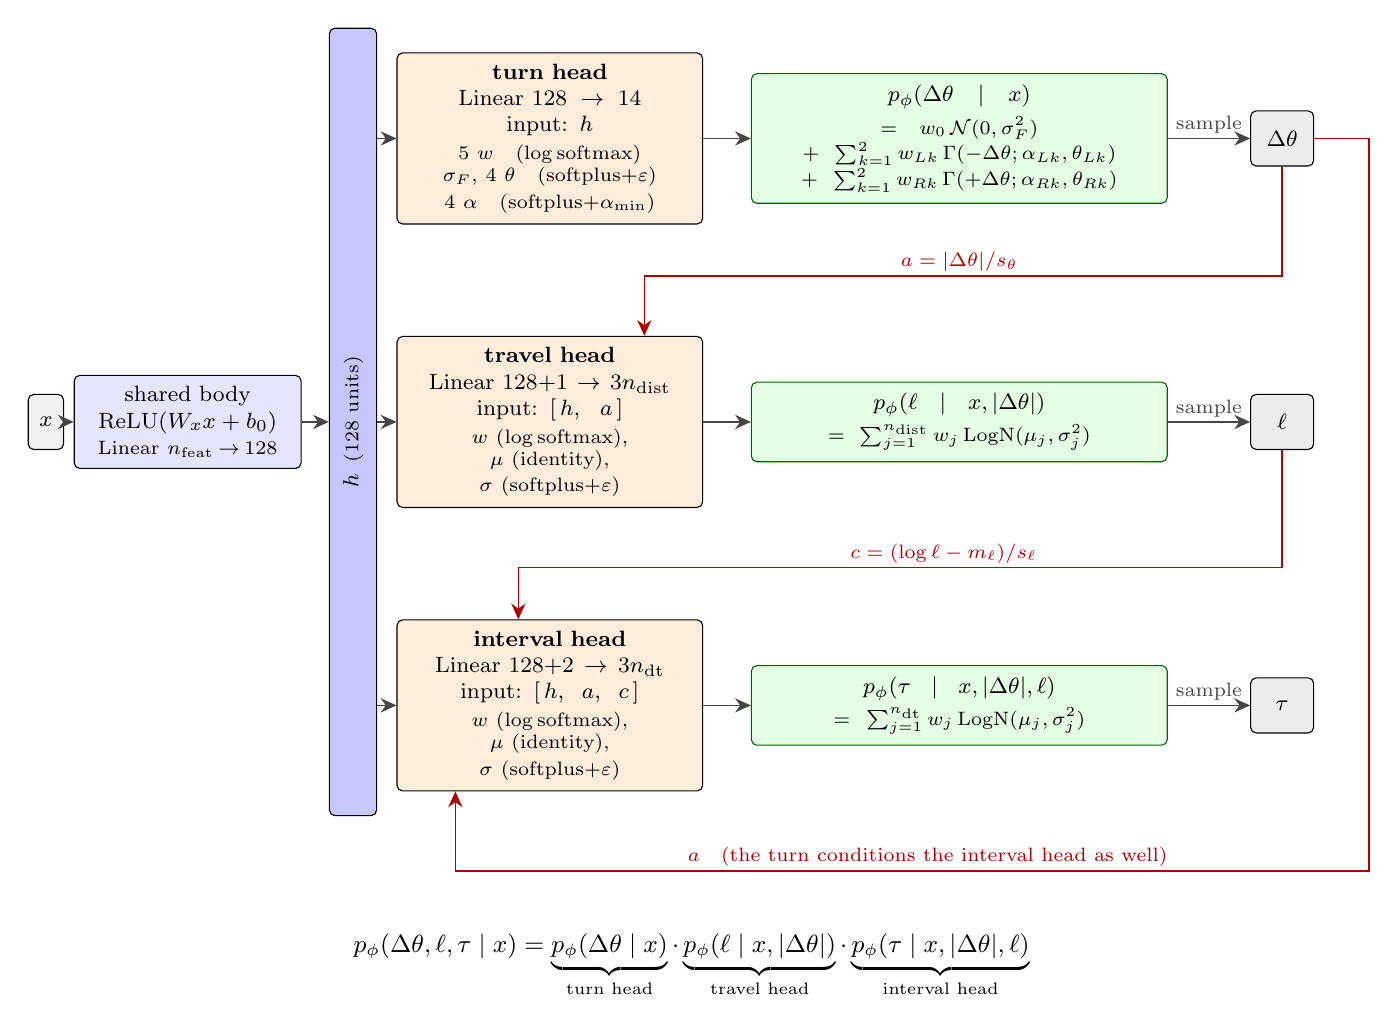
\begin{tikzpicture}[
  font=\footnotesize,
  >={Stealth[length=2mm,width=1.8mm]},
  bx/.style    = {draw, rounded corners=2pt, align=center, inner sep=4pt},
  inp/.style   = {bx, fill=gray!12, minimum height=7mm},
  bodyb/.style = {bx, fill=blue!10, text width=26mm},
  bar/.style   = {bx, fill=blue!22, minimum width=6mm, minimum height=100mm, inner sep=1pt},
  hd/.style    = {bx, fill=orange!14, text width=36mm},
  dn/.style    = {bx, fill=green!10, draw=green!40!black, text width=50mm},
  vl/.style    = {bx, fill=gray!15, minimum width=8mm, minimum height=7mm},
  fl/.style    = {->, semithick, gray!55!black},
  cd/.style    = {->, semithick, red!70!black},
  lb/.style    = {font=\scriptsize, inner sep=1.5pt},
]

% ---------------- shared trunk ----------------
\node[inp]   (x)  at (-6.2, 0) {$x$};
\node[bodyb] (bd) at (-4.4, 0) {shared body\\$\mathrm{ReLU}(W_x x + b_0)$\\
                                {\scriptsize Linear $n_{\mathrm{feat}}\!\to\!128$}};
\node[bar]   (b)  at (-2.3, 0) {\rotatebox{90}{$h$\, \scriptsize(128 units)}};

% ---------------- heads ----------------
\node[hd] (h1) at (0.2, 3.6) {\textbf{turn head}\\
  Linear $128 \to 14$\\
  input: $h$\\[2pt]
  {\scriptsize 5 $w$ \; ($\log\mathrm{softmax}$)\\
   $\sigma_F$, 4 $\theta$ \; ($\mathrm{softplus}{+}\varepsilon$)\\
   4 $\alpha$ \; ($\mathrm{softplus}{+}\alpha_{\min}$)}};
\node[hd] (h2) at (0.2, 0) {\textbf{travel head}\\
  Linear $128{+}1 \to 3n_{\mathrm{dist}}$\\
  input: $[\,h,\; a\,]$\\[2pt]
  {\scriptsize $w$ ($\log\mathrm{softmax}$), $\mu$ (identity),\\
   $\sigma$ ($\mathrm{softplus}{+}\varepsilon$)}};
\node[hd] (h3) at (0.2, -3.6) {\textbf{interval head}\\
  Linear $128{+}2 \to 3n_{\mathrm{dt}}$\\
  input: $[\,h,\; a,\; c\,]$\\[2pt]
  {\scriptsize $w$ ($\log\mathrm{softmax}$), $\mu$ (identity),\\
   $\sigma$ ($\mathrm{softplus}{+}\varepsilon$)}};

% ---------------- conditional densities ----------------
\node[dn] (d1) at (5.4, 3.6) {$p_\phi(\Delta\theta \mid x)$\\[2pt]
  {\scriptsize $= w_0\,\mathcal{N}(0,\sigma_F^2)$\\
   $+\;\sum_{k=1}^{2} w_{Lk}\,\Gamma(-\Delta\theta;\alpha_{Lk},\theta_{Lk})$\\
   $+\;\sum_{k=1}^{2} w_{Rk}\,\Gamma(+\Delta\theta;\alpha_{Rk},\theta_{Rk})$}};
\node[dn] (d2) at (5.4, 0) {$p_\phi(\ell \mid x, |\Delta\theta|)$\\[2pt]
  {\scriptsize $= \sum_{j=1}^{n_{\mathrm{dist}}} w_j\,\mathrm{LogN}(\mu_j,\sigma_j^2)$}};
\node[dn] (d3) at (5.4, -3.6) {$p_\phi(\tau \mid x, |\Delta\theta|, \ell)$\\[2pt]
  {\scriptsize $= \sum_{j=1}^{n_{\mathrm{dt}}} w_j\,\mathrm{LogN}(\mu_j,\sigma_j^2)$}};

% ---------------- emitted values ----------------
\node[vl] (v1) at (9.5, 3.6)  {$\Delta\theta$};
\node[vl] (v2) at (9.5, 0)    {$\ell$};
\node[vl] (v3) at (9.5, -3.6) {$\tau$};

% ---------------- trunk wiring ----------------
\draw[fl] (x) -- (bd);
\draw[fl] (bd) -- (b);
\draw[fl] (b.east |- h1) -- (h1.west);
\draw[fl] (b.east |- h2) -- (h2.west);
\draw[fl] (b.east |- h3) -- (h3.west);

\draw[fl] (h1.east) -- (d1.west);
\draw[fl] (h2.east) -- (d2.west);
\draw[fl] (h3.east) -- (d3.west);

\draw[fl] (d1.east) -- node[lb, above]{sample} (v1.west);
\draw[fl] (d2.east) -- node[lb, above]{sample} (v2.west);
\draw[fl] (d3.east) -- node[lb, above]{sample} (v3.west);

% ---------------- within-bout conditioners (the chain rule) ----------------
\draw[cd] (v1.south) -- (9.5,1.85) -- (1.4,1.85) -- (1.4,0 |- h2.north);
\node[lb, above, red!70!black] at (5.4,1.85) {$a = |\Delta\theta| / s_\theta$};

\draw[cd] (v2.south) -- (9.5,-1.85) -- (-0.2,-1.85) -- (-0.2,0 |- h3.north);
\node[lb, above, red!70!black] at (5.2,-1.85) {$c = (\log \ell - m_\ell)/s_\ell$};

\draw[cd] (v1.east) -- (10.6,3.6) -- (10.6,-5.7) -- (-1.0,-5.7) -- (-1.0,0 |- h3.south);
\node[lb, above, red!70!black] at (5.0,-5.7)
  {$a$ \; (the turn conditions the interval head as well)};

% ---------------- the factorisation ----------------
\node[align=center, font=\small] at (2.0,-6.9)
  {$p_\phi(\Delta\theta,\ell,\tau \mid x)
    = \underbrace{p_\phi(\Delta\theta \mid x)}_{\text{turn head}}
    \cdot \underbrace{p_\phi(\ell \mid x, |\Delta\theta|)}_{\text{travel head}}
    \cdot \underbrace{p_\phi(\tau \mid x, |\Delta\theta|, \ell)}_{\text{interval head}}$};

\end{tikzpicture}}
\caption{\textbf{Chained head architecture and the joint density it defines.}
One shared hidden layer maps the feature vector $x$ to the body representation $h$, which
every head reads. The heads do not emit probabilities: each emits the \emph{parameters} of
one conditional density (orange $\to$ green), and the joint is the chain-rule product of
the three. The red wires are the within-bout conditioners --- the travel head additionally
receives the absolute turn $a=|\Delta\theta|/s_\theta$, and the interval head receives that
and the centred log travel distance $c=(\log\ell-m_\ell)/s_\ell$, each rescaled exactly as
the corresponding history block is. During \emph{training} the red wires are teacher-forced
from the observed bout, so the three log-densities sum to the exact log joint and the loss
is $-\big[\log p_\phi(\Delta\theta\mid x)+\log p_\phi(\ell\mid x,|\Delta\theta|)
+\log p_\phi(\tau\mid x,|\Delta\theta|,\ell)\big]$ --- no bound and no approximation.
During \emph{sampling} the same wires carry the model's own draws, so a bout is generated
ancestrally, top to bottom. Only the sign-free $|\Delta\theta|$ is passed: left and right
must not change step size or timing, and feeding the sign would break the symmetry the
angle mixture enforces.}
\label{fig:architecture}
\end{figure}

% =====================================================================
\begin{figure}[p]
\centering
\resizebox{\textwidth}{!}{%
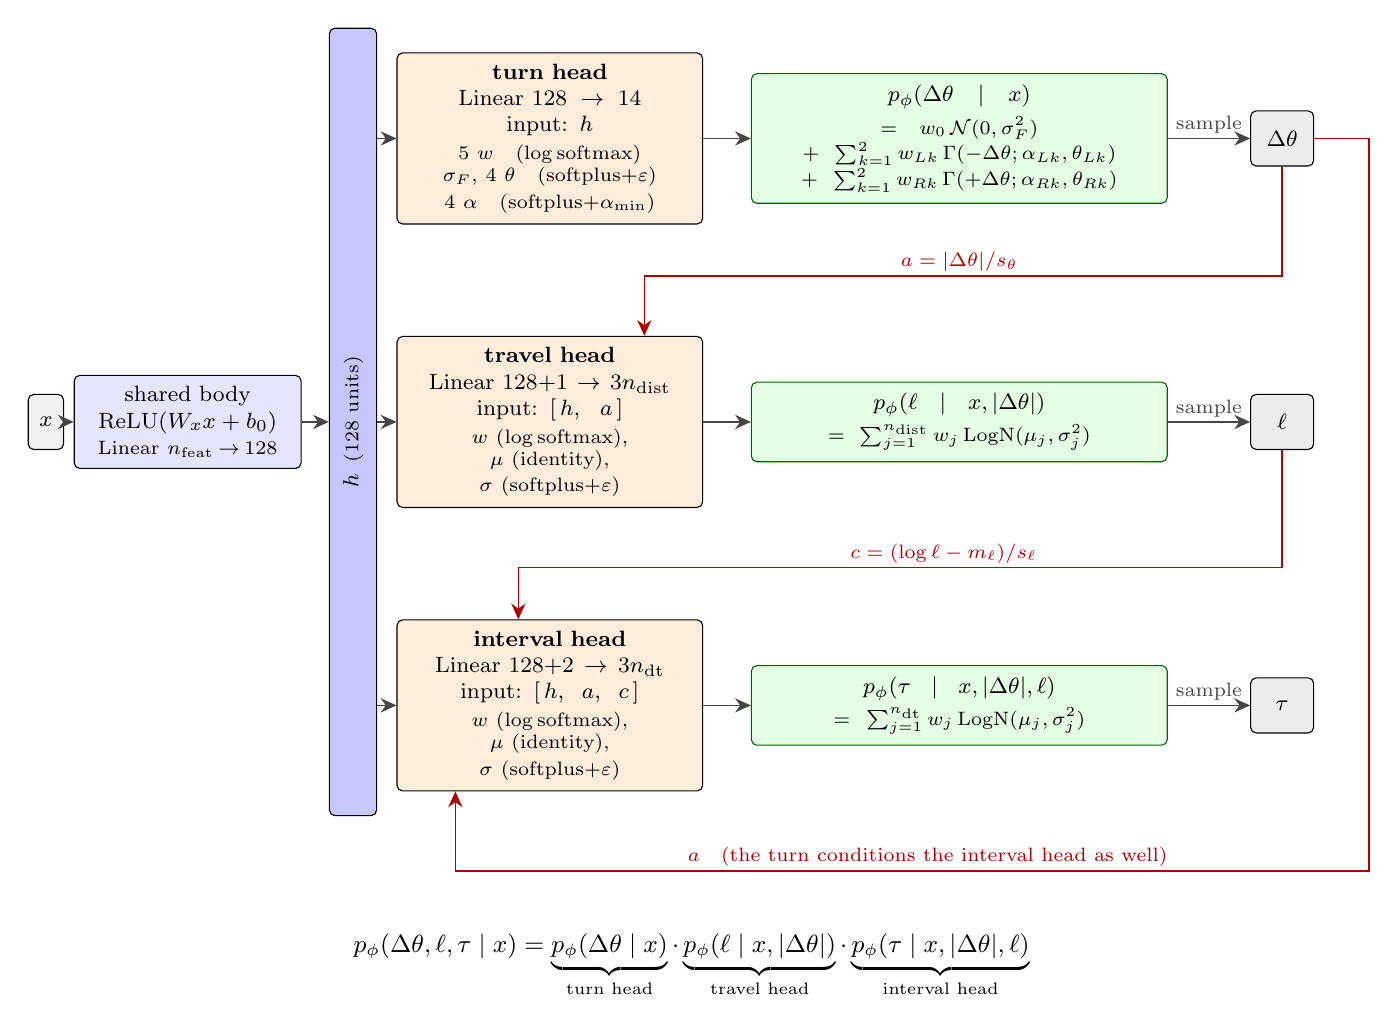
\begin{tikzpicture}[
  font=\footnotesize,
  >={Stealth[length=2mm,width=1.8mm]},
  bx/.style    = {draw, rounded corners=2pt, align=center, inner sep=4pt},
  inp/.style   = {bx, fill=gray!12, minimum height=7mm},
  bodyb/.style = {bx, fill=blue!10, text width=26mm},
  bar/.style   = {bx, fill=blue!22, minimum width=6mm, minimum height=100mm, inner sep=1pt},
  hd/.style    = {bx, fill=orange!14, text width=36mm},
  dn/.style    = {bx, fill=green!10, draw=green!40!black, text width=50mm},
  vl/.style    = {bx, fill=gray!15, minimum width=8mm, minimum height=7mm},
  fl/.style    = {->, semithick, gray!55!black},
  cd/.style    = {->, semithick, red!70!black},
  lb/.style    = {font=\scriptsize, inner sep=1.5pt},
]

% ---------------- shared trunk ----------------
\node[inp]   (x)  at (-6.2, 0) {$x$};
\node[bodyb] (bd) at (-4.4, 0) {shared body\\$\mathrm{ReLU}(W_x x + b_0)$\\
                                {\scriptsize Linear $n_{\mathrm{feat}}\!\to\!128$}};
\node[bar]   (b)  at (-2.3, 0) {\rotatebox{90}{$h$\, \scriptsize(128 units)}};

% ---------------- heads ----------------
\node[hd] (h1) at (0.2, 3.6) {\textbf{turn head}\\
  Linear $128 \to 14$\\
  input: $h$\\[2pt]
  {\scriptsize 5 $w$ \; ($\log\mathrm{softmax}$)\\
   $\sigma_F$, 4 $\theta$ \; ($\mathrm{softplus}{+}\varepsilon$)\\
   4 $\alpha$ \; ($\mathrm{softplus}{+}\alpha_{\min}$)}};
\node[hd] (h2) at (0.2, 0) {\textbf{travel head}\\
  Linear $128{+}1 \to 3n_{\mathrm{dist}}$\\
  input: $[\,h,\; a\,]$\\[2pt]
  {\scriptsize $w$ ($\log\mathrm{softmax}$), $\mu$ (identity),\\
   $\sigma$ ($\mathrm{softplus}{+}\varepsilon$)}};
\node[hd] (h3) at (0.2, -3.6) {\textbf{interval head}\\
  Linear $128{+}2 \to 3n_{\mathrm{dt}}$\\
  input: $[\,h,\; a,\; c\,]$\\[2pt]
  {\scriptsize $w$ ($\log\mathrm{softmax}$), $\mu$ (identity),\\
   $\sigma$ ($\mathrm{softplus}{+}\varepsilon$)}};

% ---------------- conditional densities ----------------
\node[dn] (d1) at (5.4, 3.6) {$p_\phi(\Delta\theta \mid x)$\\[2pt]
  {\scriptsize $= w_0\,\mathcal{N}(0,\sigma_F^2)$\\
   $+\;\sum_{k=1}^{2} w_{Lk}\,\Gamma(-\Delta\theta;\alpha_{Lk},\theta_{Lk})$\\
   $+\;\sum_{k=1}^{2} w_{Rk}\,\Gamma(+\Delta\theta;\alpha_{Rk},\theta_{Rk})$}};
\node[dn] (d2) at (5.4, 0) {$p_\phi(\ell \mid x, |\Delta\theta|)$\\[2pt]
  {\scriptsize $= \sum_{j=1}^{n_{\mathrm{dist}}} w_j\,\mathrm{LogN}(\mu_j,\sigma_j^2)$}};
\node[dn] (d3) at (5.4, -3.6) {$p_\phi(\tau \mid x, |\Delta\theta|, \ell)$\\[2pt]
  {\scriptsize $= \sum_{j=1}^{n_{\mathrm{dt}}} w_j\,\mathrm{LogN}(\mu_j,\sigma_j^2)$}};

% ---------------- emitted values ----------------
\node[vl] (v1) at (9.5, 3.6)  {$\Delta\theta$};
\node[vl] (v2) at (9.5, 0)    {$\ell$};
\node[vl] (v3) at (9.5, -3.6) {$\tau$};

% ---------------- trunk wiring ----------------
\draw[fl] (x) -- (bd);
\draw[fl] (bd) -- (b);
\draw[fl] (b.east |- h1) -- (h1.west);
\draw[fl] (b.east |- h2) -- (h2.west);
\draw[fl] (b.east |- h3) -- (h3.west);

\draw[fl] (h1.east) -- (d1.west);
\draw[fl] (h2.east) -- (d2.west);
\draw[fl] (h3.east) -- (d3.west);

\draw[fl] (d1.east) -- node[lb, above]{sample} (v1.west);
\draw[fl] (d2.east) -- node[lb, above]{sample} (v2.west);
\draw[fl] (d3.east) -- node[lb, above]{sample} (v3.west);

% ---------------- within-bout conditioners (the chain rule) ----------------
\draw[cd] (v1.south) -- (9.5,1.85) -- (1.4,1.85) -- (1.4,0 |- h2.north);
\node[lb, above, red!70!black] at (5.4,1.85) {$a = |\Delta\theta| / s_\theta$};

\draw[cd] (v2.south) -- (9.5,-1.85) -- (-0.2,-1.85) -- (-0.2,0 |- h3.north);
\node[lb, above, red!70!black] at (5.2,-1.85) {$c = (\log \ell - m_\ell)/s_\ell$};

\draw[cd] (v1.east) -- (10.6,3.6) -- (10.6,-5.7) -- (-1.0,-5.7) -- (-1.0,0 |- h3.south);
\node[lb, above, red!70!black] at (5.0,-5.7)
  {$a$ \; (the turn conditions the interval head as well)};

% ---------------- the factorisation ----------------
\node[align=center, font=\small] at (2.0,-6.9)
  {$p_\phi(\Delta\theta,\ell,\tau \mid x)
    = \underbrace{p_\phi(\Delta\theta \mid x)}_{\text{turn head}}
    \cdot \underbrace{p_\phi(\ell \mid x, |\Delta\theta|)}_{\text{travel head}}
    \cdot \underbrace{p_\phi(\tau \mid x, |\Delta\theta|, \ell)}_{\text{interval head}}$};

\end{tikzpicture}}
\caption{\textbf{Chained head architecture and the joint density it defines.}
One shared hidden layer maps the feature vector $x$ to the body representation $h$, which
every head reads. The heads do not emit probabilities: each emits the \emph{parameters} of
one conditional density (orange $\to$ green), and the joint is the chain-rule product of
the three. The red wires are the within-bout conditioners --- the travel head additionally
receives the absolute turn $a=|\Delta\theta|/s_\theta$, and the interval head receives that
and the centred log travel distance $c=(\log\ell-m_\ell)/s_\ell$, each rescaled exactly as
the corresponding history block is. During \emph{training} the red wires are teacher-forced
from the observed bout, so the three log-densities sum to the exact log joint and the loss
is $-\big[\log p_\phi(\Delta\theta\mid x)+\log p_\phi(\ell\mid x,|\Delta\theta|)
+\log p_\phi(\tau\mid x,|\Delta\theta|,\ell)\big]$ --- no bound and no approximation.
During \emph{sampling} the same wires carry the model's own draws, so a bout is generated
ancestrally, top to bottom. Only the sign-free $|\Delta\theta|$ is passed: left and right
must not change step size or timing, and feeding the sign would break the symmetry the
angle mixture enforces.}
\label{fig:architecture}
\end{figure}

% =====================================================================
\begin{figure}[p]
\centering
\resizebox{\textwidth}{!}{%
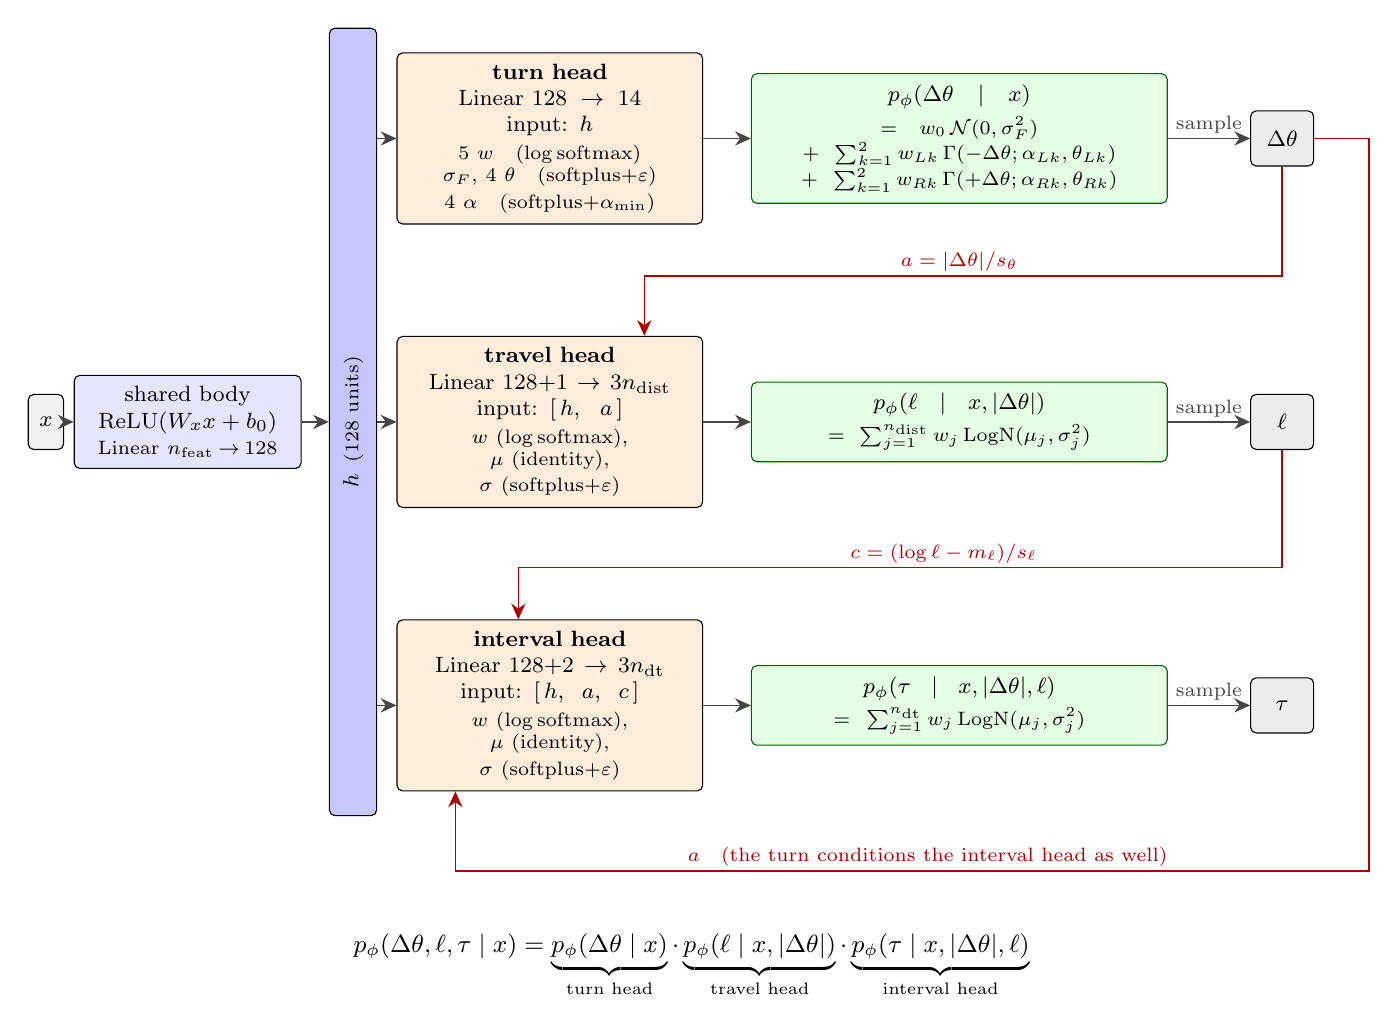
\begin{tikzpicture}[
  font=\footnotesize,
  >={Stealth[length=2mm,width=1.8mm]},
  bx/.style    = {draw, rounded corners=2pt, align=center, inner sep=4pt},
  inp/.style   = {bx, fill=gray!12, minimum height=7mm},
  bodyb/.style = {bx, fill=blue!10, text width=26mm},
  bar/.style   = {bx, fill=blue!22, minimum width=6mm, minimum height=100mm, inner sep=1pt},
  hd/.style    = {bx, fill=orange!14, text width=36mm},
  dn/.style    = {bx, fill=green!10, draw=green!40!black, text width=50mm},
  vl/.style    = {bx, fill=gray!15, minimum width=8mm, minimum height=7mm},
  fl/.style    = {->, semithick, gray!55!black},
  cd/.style    = {->, semithick, red!70!black},
  lb/.style    = {font=\scriptsize, inner sep=1.5pt},
]

% ---------------- shared trunk ----------------
\node[inp]   (x)  at (-6.2, 0) {$x$};
\node[bodyb] (bd) at (-4.4, 0) {shared body\\$\mathrm{ReLU}(W_x x + b_0)$\\
                                {\scriptsize Linear $n_{\mathrm{feat}}\!\to\!128$}};
\node[bar]   (b)  at (-2.3, 0) {\rotatebox{90}{$h$\, \scriptsize(128 units)}};

% ---------------- heads ----------------
\node[hd] (h1) at (0.2, 3.6) {\textbf{turn head}\\
  Linear $128 \to 14$\\
  input: $h$\\[2pt]
  {\scriptsize 5 $w$ \; ($\log\mathrm{softmax}$)\\
   $\sigma_F$, 4 $\theta$ \; ($\mathrm{softplus}{+}\varepsilon$)\\
   4 $\alpha$ \; ($\mathrm{softplus}{+}\alpha_{\min}$)}};
\node[hd] (h2) at (0.2, 0) {\textbf{travel head}\\
  Linear $128{+}1 \to 3n_{\mathrm{dist}}$\\
  input: $[\,h,\; a\,]$\\[2pt]
  {\scriptsize $w$ ($\log\mathrm{softmax}$), $\mu$ (identity),\\
   $\sigma$ ($\mathrm{softplus}{+}\varepsilon$)}};
\node[hd] (h3) at (0.2, -3.6) {\textbf{interval head}\\
  Linear $128{+}2 \to 3n_{\mathrm{dt}}$\\
  input: $[\,h,\; a,\; c\,]$\\[2pt]
  {\scriptsize $w$ ($\log\mathrm{softmax}$), $\mu$ (identity),\\
   $\sigma$ ($\mathrm{softplus}{+}\varepsilon$)}};

% ---------------- conditional densities ----------------
\node[dn] (d1) at (5.4, 3.6) {$p_\phi(\Delta\theta \mid x)$\\[2pt]
  {\scriptsize $= w_0\,\mathcal{N}(0,\sigma_F^2)$\\
   $+\;\sum_{k=1}^{2} w_{Lk}\,\Gamma(-\Delta\theta;\alpha_{Lk},\theta_{Lk})$\\
   $+\;\sum_{k=1}^{2} w_{Rk}\,\Gamma(+\Delta\theta;\alpha_{Rk},\theta_{Rk})$}};
\node[dn] (d2) at (5.4, 0) {$p_\phi(\ell \mid x, |\Delta\theta|)$\\[2pt]
  {\scriptsize $= \sum_{j=1}^{n_{\mathrm{dist}}} w_j\,\mathrm{LogN}(\mu_j,\sigma_j^2)$}};
\node[dn] (d3) at (5.4, -3.6) {$p_\phi(\tau \mid x, |\Delta\theta|, \ell)$\\[2pt]
  {\scriptsize $= \sum_{j=1}^{n_{\mathrm{dt}}} w_j\,\mathrm{LogN}(\mu_j,\sigma_j^2)$}};

% ---------------- emitted values ----------------
\node[vl] (v1) at (9.5, 3.6)  {$\Delta\theta$};
\node[vl] (v2) at (9.5, 0)    {$\ell$};
\node[vl] (v3) at (9.5, -3.6) {$\tau$};

% ---------------- trunk wiring ----------------
\draw[fl] (x) -- (bd);
\draw[fl] (bd) -- (b);
\draw[fl] (b.east |- h1) -- (h1.west);
\draw[fl] (b.east |- h2) -- (h2.west);
\draw[fl] (b.east |- h3) -- (h3.west);

\draw[fl] (h1.east) -- (d1.west);
\draw[fl] (h2.east) -- (d2.west);
\draw[fl] (h3.east) -- (d3.west);

\draw[fl] (d1.east) -- node[lb, above]{sample} (v1.west);
\draw[fl] (d2.east) -- node[lb, above]{sample} (v2.west);
\draw[fl] (d3.east) -- node[lb, above]{sample} (v3.west);

% ---------------- within-bout conditioners (the chain rule) ----------------
\draw[cd] (v1.south) -- (9.5,1.85) -- (1.4,1.85) -- (1.4,0 |- h2.north);
\node[lb, above, red!70!black] at (5.4,1.85) {$a = |\Delta\theta| / s_\theta$};

\draw[cd] (v2.south) -- (9.5,-1.85) -- (-0.2,-1.85) -- (-0.2,0 |- h3.north);
\node[lb, above, red!70!black] at (5.2,-1.85) {$c = (\log \ell - m_\ell)/s_\ell$};

\draw[cd] (v1.east) -- (10.6,3.6) -- (10.6,-5.7) -- (-1.0,-5.7) -- (-1.0,0 |- h3.south);
\node[lb, above, red!70!black] at (5.0,-5.7)
  {$a$ \; (the turn conditions the interval head as well)};

% ---------------- the factorisation ----------------
\node[align=center, font=\small] at (2.0,-6.9)
  {$p_\phi(\Delta\theta,\ell,\tau \mid x)
    = \underbrace{p_\phi(\Delta\theta \mid x)}_{\text{turn head}}
    \cdot \underbrace{p_\phi(\ell \mid x, |\Delta\theta|)}_{\text{travel head}}
    \cdot \underbrace{p_\phi(\tau \mid x, |\Delta\theta|, \ell)}_{\text{interval head}}$};

\end{tikzpicture}}
\caption{\textbf{Chained head architecture and the joint density it defines.}
One shared hidden layer maps the feature vector $x$ to the body representation $h$, which
every head reads. The heads do not emit probabilities: each emits the \emph{parameters} of
one conditional density (orange $\to$ green), and the joint is the chain-rule product of
the three. The red wires are the within-bout conditioners --- the travel head additionally
receives the absolute turn $a=|\Delta\theta|/s_\theta$, and the interval head receives that
and the centred log travel distance $c=(\log\ell-m_\ell)/s_\ell$, each rescaled exactly as
the corresponding history block is. During \emph{training} the red wires are teacher-forced
from the observed bout, so the three log-densities sum to the exact log joint and the loss
is $-\big[\log p_\phi(\Delta\theta\mid x)+\log p_\phi(\ell\mid x,|\Delta\theta|)
+\log p_\phi(\tau\mid x,|\Delta\theta|,\ell)\big]$ --- no bound and no approximation.
During \emph{sampling} the same wires carry the model's own draws, so a bout is generated
ancestrally, top to bottom. Only the sign-free $|\Delta\theta|$ is passed: left and right
must not change step size or timing, and feeding the sign would break the symmetry the
angle mixture enforces.}
\label{fig:architecture}
\end{figure}

\clearpage
% =====================================================================
%  Nomenclature for fig_architecture.tex.
%  Requires: \usepackage{booktabs}  \usepackage{array}  \usepackage{amsmath}
%  Use with: % =====================================================================
%  Nomenclature for fig_architecture.tex.
%  Requires: \usepackage{booktabs}  \usepackage{array}  \usepackage{amsmath}
%  Use with: % =====================================================================
%  Nomenclature for fig_architecture.tex.
%  Requires: \usepackage{booktabs}  \usepackage{array}  \usepackage{amsmath}
%  Use with: \input{fig_architecture_symbols}
% =====================================================================
\begin{table}[t]
\centering\small
\renewcommand{\arraystretch}{1.18}
\begin{tabular}{@{}l l p{0.56\linewidth}@{}}
\toprule
\textbf{symbol} & \textbf{space} & \textbf{meaning}\\
\midrule
\multicolumn{3}{@{}l}{\emph{Shared trunk}}\\
$x$        & $\mathbb{R}^{n_{\mathrm{feat}}}$ & input feature vector for one bout: the
             concatenated turn-history, symbol, stimulus, border, adaptation and
             kinematic-history blocks; $n_{\mathrm{feat}}$ is their total width\\
$W_x$      & $\mathbb{R}^{128\times n_{\mathrm{feat}}}$ & weight matrix of the single hidden layer\\
$b_0$      & $\mathbb{R}^{128}$ & bias vector of that layer\\
$h$        & $\mathbb{R}^{128}$ & hidden (body) representation $h=\mathrm{ReLU}(W_x x + b_0)$,
             read by all three heads; $128$ is the layer width\\
$\phi$     & --- & all trainable parameters ($W_x$, $b_0$ and the three head weight matrices
             and biases); the subscript in $p_\phi$\\
\addlinespace
\multicolumn{3}{@{}l}{\emph{The three emitted channels of a bout}}\\
$\Delta\theta$ & $(-180,180]$ deg & signed reorientation angle (the turn)\\
$\ell$     & $(0,\infty)$ px & travel distance of the bout, onset to onset\\
$\tau$     & $(0,\infty)$ s  & inter-bout interval\\
\addlinespace
\multicolumn{3}{@{}l}{\emph{Within-bout conditioners (the chain-rule wires)}}\\
$a$        & $\mathbb{R}_{\ge 0}$ & rescaled absolute turn, $a=|\Delta\theta|/s_\theta$\\
$c$        & $\mathbb{R}$ & centred log travel distance, $c=(\log\ell-m_\ell)/s_\ell$\\
$s_\theta$ & $>0$ & turn scale, $\max(\mathrm{sd}(\Delta\theta),1)$ on the training fold\\
$m_\ell,\,s_\ell$ & $\mathbb{R},>0$ & mean and sd of $\log\ell$ on the training fold\\
\addlinespace
\multicolumn{3}{@{}l}{\emph{Turn-head parameters (14 raw outputs)}}\\
$w_0,w_{L1},w_{L2},w_{R1},w_{R2}$ & simplex & the five mixture weights ($\log\mathrm{softmax}$)\\
$\sigma_F$ & $>0$ & standard deviation of the forward Normal, centred at $0$\\
$\alpha_{Lk},\theta_{Lk}$ & $\ge\alpha_{\min},>0$ & shape and scale of left Gamma $k$, on $-\Delta\theta$\\
$\alpha_{Rk},\theta_{Rk}$ & $\ge\alpha_{\min},>0$ & shape and scale of right Gamma $k$, on $+\Delta\theta$\\
\addlinespace
\multicolumn{3}{@{}l}{\emph{Travel- and interval-head parameters}}\\
$n_{\mathrm{dist}},\,n_{\mathrm{dt}}$ & $\mathbb{N}$ & number of log-normal components (2 and 3)\\
$w_j,\mu_j,\sigma_j$ & simplex, $\mathbb{R}$, $>0$ & weight, log-scale location and log-scale
             spread of component $j$; $3n$ raw outputs per head\\
\addlinespace
\multicolumn{3}{@{}l}{\emph{Constants and distributions}}\\
$\varepsilon$ & $10^{-12}$ & softplus floor keeping every scale strictly positive\\
$\alpha_{\min}$ & $1$ & floor on the Gamma shape, so no component diverges at $\Delta\theta\!\to\!0$\\
$\mathcal{N}(0,\sigma^2)$ & --- & Normal density\\
$\Gamma(u;\alpha,\theta)$ & --- & Gamma density on $u>0$, shape $\alpha$, scale $\theta$\\
$\mathrm{LogN}(\mu,\sigma^2)$ & --- & log-normal: $\log X\sim\mathcal{N}(\mu,\sigma^2)$\\
\bottomrule
\end{tabular}
\caption{Symbols used in Fig.~\ref{fig:architecture}.}
\label{tab:architecture-symbols}
\end{table}

% =====================================================================
\begin{table}[t]
\centering\small
\renewcommand{\arraystretch}{1.18}
\begin{tabular}{@{}l l p{0.56\linewidth}@{}}
\toprule
\textbf{symbol} & \textbf{space} & \textbf{meaning}\\
\midrule
\multicolumn{3}{@{}l}{\emph{Shared trunk}}\\
$x$        & $\mathbb{R}^{n_{\mathrm{feat}}}$ & input feature vector for one bout: the
             concatenated turn-history, symbol, stimulus, border, adaptation and
             kinematic-history blocks; $n_{\mathrm{feat}}$ is their total width\\
$W_x$      & $\mathbb{R}^{128\times n_{\mathrm{feat}}}$ & weight matrix of the single hidden layer\\
$b_0$      & $\mathbb{R}^{128}$ & bias vector of that layer\\
$h$        & $\mathbb{R}^{128}$ & hidden (body) representation $h=\mathrm{ReLU}(W_x x + b_0)$,
             read by all three heads; $128$ is the layer width\\
$\phi$     & --- & all trainable parameters ($W_x$, $b_0$ and the three head weight matrices
             and biases); the subscript in $p_\phi$\\
\addlinespace
\multicolumn{3}{@{}l}{\emph{The three emitted channels of a bout}}\\
$\Delta\theta$ & $(-180,180]$ deg & signed reorientation angle (the turn)\\
$\ell$     & $(0,\infty)$ px & travel distance of the bout, onset to onset\\
$\tau$     & $(0,\infty)$ s  & inter-bout interval\\
\addlinespace
\multicolumn{3}{@{}l}{\emph{Within-bout conditioners (the chain-rule wires)}}\\
$a$        & $\mathbb{R}_{\ge 0}$ & rescaled absolute turn, $a=|\Delta\theta|/s_\theta$\\
$c$        & $\mathbb{R}$ & centred log travel distance, $c=(\log\ell-m_\ell)/s_\ell$\\
$s_\theta$ & $>0$ & turn scale, $\max(\mathrm{sd}(\Delta\theta),1)$ on the training fold\\
$m_\ell,\,s_\ell$ & $\mathbb{R},>0$ & mean and sd of $\log\ell$ on the training fold\\
\addlinespace
\multicolumn{3}{@{}l}{\emph{Turn-head parameters (14 raw outputs)}}\\
$w_0,w_{L1},w_{L2},w_{R1},w_{R2}$ & simplex & the five mixture weights ($\log\mathrm{softmax}$)\\
$\sigma_F$ & $>0$ & standard deviation of the forward Normal, centred at $0$\\
$\alpha_{Lk},\theta_{Lk}$ & $\ge\alpha_{\min},>0$ & shape and scale of left Gamma $k$, on $-\Delta\theta$\\
$\alpha_{Rk},\theta_{Rk}$ & $\ge\alpha_{\min},>0$ & shape and scale of right Gamma $k$, on $+\Delta\theta$\\
\addlinespace
\multicolumn{3}{@{}l}{\emph{Travel- and interval-head parameters}}\\
$n_{\mathrm{dist}},\,n_{\mathrm{dt}}$ & $\mathbb{N}$ & number of log-normal components (2 and 3)\\
$w_j,\mu_j,\sigma_j$ & simplex, $\mathbb{R}$, $>0$ & weight, log-scale location and log-scale
             spread of component $j$; $3n$ raw outputs per head\\
\addlinespace
\multicolumn{3}{@{}l}{\emph{Constants and distributions}}\\
$\varepsilon$ & $10^{-12}$ & softplus floor keeping every scale strictly positive\\
$\alpha_{\min}$ & $1$ & floor on the Gamma shape, so no component diverges at $\Delta\theta\!\to\!0$\\
$\mathcal{N}(0,\sigma^2)$ & --- & Normal density\\
$\Gamma(u;\alpha,\theta)$ & --- & Gamma density on $u>0$, shape $\alpha$, scale $\theta$\\
$\mathrm{LogN}(\mu,\sigma^2)$ & --- & log-normal: $\log X\sim\mathcal{N}(\mu,\sigma^2)$\\
\bottomrule
\end{tabular}
\caption{Symbols used in Fig.~\ref{fig:architecture}.}
\label{tab:architecture-symbols}
\end{table}

% =====================================================================
\begin{table}[t]
\centering\small
\renewcommand{\arraystretch}{1.18}
\begin{tabular}{@{}l l p{0.56\linewidth}@{}}
\toprule
\textbf{symbol} & \textbf{space} & \textbf{meaning}\\
\midrule
\multicolumn{3}{@{}l}{\emph{Shared trunk}}\\
$x$        & $\mathbb{R}^{n_{\mathrm{feat}}}$ & input feature vector for one bout: the
             concatenated turn-history, symbol, stimulus, border, adaptation and
             kinematic-history blocks; $n_{\mathrm{feat}}$ is their total width\\
$W_x$      & $\mathbb{R}^{128\times n_{\mathrm{feat}}}$ & weight matrix of the single hidden layer\\
$b_0$      & $\mathbb{R}^{128}$ & bias vector of that layer\\
$h$        & $\mathbb{R}^{128}$ & hidden (body) representation $h=\mathrm{ReLU}(W_x x + b_0)$,
             read by all three heads; $128$ is the layer width\\
$\phi$     & --- & all trainable parameters ($W_x$, $b_0$ and the three head weight matrices
             and biases); the subscript in $p_\phi$\\
\addlinespace
\multicolumn{3}{@{}l}{\emph{The three emitted channels of a bout}}\\
$\Delta\theta$ & $(-180,180]$ deg & signed reorientation angle (the turn)\\
$\ell$     & $(0,\infty)$ px & travel distance of the bout, onset to onset\\
$\tau$     & $(0,\infty)$ s  & inter-bout interval\\
\addlinespace
\multicolumn{3}{@{}l}{\emph{Within-bout conditioners (the chain-rule wires)}}\\
$a$        & $\mathbb{R}_{\ge 0}$ & rescaled absolute turn, $a=|\Delta\theta|/s_\theta$\\
$c$        & $\mathbb{R}$ & centred log travel distance, $c=(\log\ell-m_\ell)/s_\ell$\\
$s_\theta$ & $>0$ & turn scale, $\max(\mathrm{sd}(\Delta\theta),1)$ on the training fold\\
$m_\ell,\,s_\ell$ & $\mathbb{R},>0$ & mean and sd of $\log\ell$ on the training fold\\
\addlinespace
\multicolumn{3}{@{}l}{\emph{Turn-head parameters (14 raw outputs)}}\\
$w_0,w_{L1},w_{L2},w_{R1},w_{R2}$ & simplex & the five mixture weights ($\log\mathrm{softmax}$)\\
$\sigma_F$ & $>0$ & standard deviation of the forward Normal, centred at $0$\\
$\alpha_{Lk},\theta_{Lk}$ & $\ge\alpha_{\min},>0$ & shape and scale of left Gamma $k$, on $-\Delta\theta$\\
$\alpha_{Rk},\theta_{Rk}$ & $\ge\alpha_{\min},>0$ & shape and scale of right Gamma $k$, on $+\Delta\theta$\\
\addlinespace
\multicolumn{3}{@{}l}{\emph{Travel- and interval-head parameters}}\\
$n_{\mathrm{dist}},\,n_{\mathrm{dt}}$ & $\mathbb{N}$ & number of log-normal components (2 and 3)\\
$w_j,\mu_j,\sigma_j$ & simplex, $\mathbb{R}$, $>0$ & weight, log-scale location and log-scale
             spread of component $j$; $3n$ raw outputs per head\\
\addlinespace
\multicolumn{3}{@{}l}{\emph{Constants and distributions}}\\
$\varepsilon$ & $10^{-12}$ & softplus floor keeping every scale strictly positive\\
$\alpha_{\min}$ & $1$ & floor on the Gamma shape, so no component diverges at $\Delta\theta\!\to\!0$\\
$\mathcal{N}(0,\sigma^2)$ & --- & Normal density\\
$\Gamma(u;\alpha,\theta)$ & --- & Gamma density on $u>0$, shape $\alpha$, scale $\theta$\\
$\mathrm{LogN}(\mu,\sigma^2)$ & --- & log-normal: $\log X\sim\mathcal{N}(\mu,\sigma^2)$\\
\bottomrule
\end{tabular}
\caption{Symbols used in Fig.~\ref{fig:architecture}.}
\label{tab:architecture-symbols}
\end{table}

\clearpage
\input{fig_architecture-latent}
\clearpage


\end{document}
